\documentclass[11pt,letterpaper]{article}
\usepackage[margin=.72in]{geometry}
\usepackage[T1]{fontenc}
\usepackage{lmodern,microtype,booktabs,array,graphicx,pdflscape,xcolor,amsmath,hyperref}
\hypersetup{colorlinks=true,urlcolor=blue,linkcolor=blue,pdftitle={Financial facts need their full context}}
\setlength{\parindent}{0pt}\setlength{\parskip}{6pt}
\newcommand{\heading}[1]{\vspace{4pt}{\large\bfseries #1}\par}
\newcommand{\BoundA}{247}
\newcommand{\BoundB}{27}
\newcommand{\BoundC}{220}
\newcommand{\BoundD}{10}
\newcommand{\BoundE}{16}
\newcommand{\BoundF}{210}
\newcommand{\BoundG}{37}
\newcommand{\BoundH}{215}
\newcommand{\BoundI}{3}
\newcommand{\BoundJ}{18}
\newcommand{\BoundK}{0}
\newcommand{\BoundL}{27}
\newcommand{\BoundM}{220}
\newcommand{\BoundN}{15}
\newcommand{\BoundO}{215}
\newcommand{\BoundP}{10}
\newcommand{\BoundQ}{16}
\newcommand{\BoundR}{37}
\newcommand{\BoundS}{210}
\newcommand{\BoundT}{17}
\newcommand{\BoundU}{203}
\newcommand{\BoundV}{0}
\newcommand{\BoundW}{24}
\newcommand{\BoundX}{37}
\newcommand{\BoundY}{210}
\newcommand{\BoundZ}{17}
\newcommand{\BoundAA}{203}
\newcommand{\BoundAB}{0}
\newcommand{\BoundAC}{24}
\newcommand{\BoundAD}{37}
\newcommand{\BoundAE}{210}
\newcommand{\BoundAF}{17}
\newcommand{\BoundAG}{203}
\newcommand{\BoundAH}{0}
\newcommand{\BoundAI}{24}
\newcommand{\BoundAJ}{247}
\newcommand{\BoundAK}{0}
\newcommand{\BoundAL}{0}
\newcommand{\BoundAM}{0}
\newcommand{\BoundAN}{0}
\newcommand{\BoundAO}{0}
\newcommand{\BoundAP}{247}
\newcommand{\BoundAQ}{0}
\newcommand{\BoundAR}{0}
\newcommand{\BoundAS}{0}
\newcommand{\BoundAT}{0}
\newcommand{\BoundAU}{0}
\newcommand{\BoundAV}{11}
\newcommand{\BoundAW}{3}
\newcommand{\BoundAX}{8}
\newcommand{\BoundAY}{8}
\newcommand{\BoundAZ}{11}
\newcommand{\BoundBA}{0}
\newcommand{\BoundBB}{0}
\newcommand{\BoundBC}{0}
\newcommand{\BoundBD}{0}
\newcommand{\BoundBE}{0}
\newcommand{\BoundBF}{4}
\newcommand{\BoundBG}{2}
\newcommand{\BoundBH}{2}
\newcommand{\BoundBI}{2}
\newcommand{\BoundBJ}{4}
\newcommand{\BoundBK}{88}
\newcommand{\BoundBL}{2}
\newcommand{\BoundBM}{86}
\newcommand{\BoundBN}{86}
\newcommand{\BoundBO}{88}
\newcommand{\BoundBP}{16}
\newcommand{\BoundBQ}{2}
\newcommand{\BoundBR}{14}
\newcommand{\BoundBS}{14}
\newcommand{\BoundBT}{16}
\newcommand{\BoundBU}{0}
\newcommand{\BoundBV}{0}
\newcommand{\BoundBW}{0}
\newcommand{\BoundBX}{0}
\newcommand{\BoundBY}{0}
\newcommand{\BoundBZ}{2}
\newcommand{\BoundCA}{2}
\newcommand{\BoundCB}{0}
\newcommand{\BoundCC}{0}
\newcommand{\BoundCD}{2}
\newcommand{\BoundCE}{2}
\newcommand{\BoundCF}{2}
\newcommand{\BoundCG}{0}
\newcommand{\BoundCH}{0}
\newcommand{\BoundCI}{2}
\newcommand{\BoundCJ}{8}
\newcommand{\BoundCK}{2}
\newcommand{\BoundCL}{6}
\newcommand{\BoundCM}{4}
\newcommand{\BoundCN}{8}
\newcommand{\BoundCO}{48}
\newcommand{\BoundCP}{2}
\newcommand{\BoundCQ}{46}
\newcommand{\BoundCR}{46}
\newcommand{\BoundCS}{48}
\newcommand{\BoundCT}{0}
\newcommand{\BoundCU}{0}
\newcommand{\BoundCV}{0}
\newcommand{\BoundCW}{0}
\newcommand{\BoundCX}{0}
\newcommand{\BoundCY}{0}
\newcommand{\BoundCZ}{0}
\newcommand{\BoundDA}{0}
\newcommand{\BoundDB}{0}
\newcommand{\BoundDC}{0}
\newcommand{\BoundDD}{2}
\newcommand{\BoundDE}{2}
\newcommand{\BoundDF}{0}
\newcommand{\BoundDG}{0}
\newcommand{\BoundDH}{2}
\newcommand{\BoundDI}{2}
\newcommand{\BoundDJ}{2}
\newcommand{\BoundDK}{0}
\newcommand{\BoundDL}{0}
\newcommand{\BoundDM}{2}
\newcommand{\BoundDN}{6}
\newcommand{\BoundDO}{3}
\newcommand{\BoundDP}{3}
\newcommand{\BoundDQ}{0}
\newcommand{\BoundDR}{6}
\newcommand{\BoundDS}{58}
\newcommand{\BoundDT}{3}
\newcommand{\BoundDU}{55}
\newcommand{\BoundDV}{55}
\newcommand{\BoundDW}{58}
\newcommand{\BoundDX}{0}
\newcommand{\BoundDY}{0}
\newcommand{\BoundDZ}{0}
\newcommand{\BoundEA}{0}
\newcommand{\BoundEB}{0}
\newcommand{\BoundEC}{0}
\newcommand{\BoundED}{0}
\newcommand{\BoundEE}{0}
\newcommand{\BoundEF}{0}
\newcommand{\BoundEG}{0}
\newcommand{\BoundEH}{108}
\newcommand{\BoundEI}{632}
\newcommand{\BoundEJ}{1,482}
\newcommand{\BoundEK}{6,516}
\newcommand{\BoundEL}{87,871}
\newcommand{\BoundEM}{731,170}
\newcommand{\BoundEN}{3,905,397}
\newcommand{\BoundEO}{373}
\newcommand{\BoundEP}{2,232}
\newcommand{\BoundEQ}{2,039}
\newcommand{\BoundER}{24}
\newcommand{\BoundES}{32}
\newcommand{\BoundET}{3.10.11}
\newcommand{\BoundEU}{3.12.14}
\newcommand{\BoundEV}{54}
\newcommand{\BoundEW}{216}
\newcommand{\BoundEX}{25}
\begin{document}
{\LARGE\bfseries Financial facts need their full context\par}
\vspace{5pt}
Independent research program\hfill 31 October 2026 UTC\\
\textit{Not peer reviewed. One current SEC extract; fixed relational-key comparisons.}

\heading{Practical finding}
A company, tag and period-end date do not uniquely identify a financial fact. In this fixed cohort, that short key collapses \BoundA{} facts into \BoundB{} groups. A one-row-per-key join would discard \BoundC{} distinct source contexts.

The short key mixes durations in \BoundD{} groups and segment/coregistrant contexts in \BoundE{} groups. Adding duration still leaves \BoundF{} extra contexts within \BoundG{} groups. Retaining segment/coregistrant identity separates every observed fact here. Accession remains part of the full source key even though each company has only one selected filing in this archive.

An authored naive-winner simulation finds \BoundH{} source facts with a different numeric value from their short-key winner. Different durations or dimensions can describe different quantities. This is not a count of verified restatements, financial losses or historical feature leakage.

\heading{Recommended use}
Carry accession, tag, taxonomy version, period, duration, unit, segment and coregistrant identity through a financial-data join. Require a complete context before returning a qualified fact; abstain when it is absent or ambiguous. Classify context differences before interpreting a changed value as a revision.

The implementation exercise retains a useful failed assumption: an Apple example requested a 2026 taxonomy, while the source uses a 2025 taxonomy. The lookup correctly abstains. A separately labeled post-analysis positive control uses the actual version and returns a qualified source value. Filing year is insufficient evidence for taxonomy version.

\heading{Fixed source and scope}
The official current 2026 Q3 face-financial archive supplies \BoundI{} selected filings from Apple, Microsoft and Walmart. The protocol fixed those CIKs, six standard financial tags and all six key specifications before retrieval. All \BoundJ{} company/tag cells are retained, including empty cells; this is a convenience cohort.

The original broad historical restatement/model-leakage question remains unexecuted. There are \BoundK{} repeated-context observations across accessions in this selected cohort. That absence cannot establish that historical financial values are stable.
\newpage
{\Large\bfseries Complete fixed key accounts\par}
{\small\setlength{\tabcolsep}{5pt}
\begin{tabular}{@{}lrrrrrr@{}}\toprule
Key & Groups & Extra contexts & Conflicts & Value differences & Mixed duration & Mixed segment\\\midrule
K0 & \BoundL{} & \BoundM{} & \BoundN{} & \BoundO{} & \BoundP{} & \BoundQ{} \\
K1 & \BoundR{} & \BoundS{} & \BoundT{} & \BoundU{} & \BoundV{} & \BoundW{} \\
K2 & \BoundX{} & \BoundY{} & \BoundZ{} & \BoundAA{} & \BoundAB{} & \BoundAC{} \\
K3 & \BoundAD{} & \BoundAE{} & \BoundAF{} & \BoundAG{} & \BoundAH{} & \BoundAI{} \\
K4 & \BoundAJ{} & \BoundAK{} & \BoundAL{} & \BoundAM{} & \BoundAN{} & \BoundAO{} \\
K5 & \BoundAP{} & \BoundAQ{} & \BoundAR{} & \BoundAS{} & \BoundAT{} & \BoundAU{} \\
\bottomrule\end{tabular}}

K0 uses CIK, tag and rounded end date. K1 adds duration, K2 unit, K3 taxonomy, K4 segment/coregistrant identity and K5 accession. All units and taxonomy versions remain explicit even where they do not split a group in this cohort. Conflicting-group counts need not decline at every step: a larger group can split into several groups that each contain differing values.

\heading{All company/tag cells, including zero coverage}
{\small\setlength{\tabcolsep}{5pt}
\begin{tabular}{@{}llrrrrr@{}}\toprule
Company & Tag label & Facts & K0 groups & K0 extra & K0 value differences & K4 groups\\\midrule
Walmart & Assets & \BoundAV{} & \BoundAW{} & \BoundAX{} & \BoundAY{} & \BoundAZ{} \\
Walmart & Liabilities & \BoundBA{} & \BoundBB{} & \BoundBC{} & \BoundBD{} & \BoundBE{} \\
Walmart & Net income & \BoundBF{} & \BoundBG{} & \BoundBH{} & \BoundBI{} & \BoundBJ{} \\
Walmart & Contract revenue & \BoundBK{} & \BoundBL{} & \BoundBM{} & \BoundBN{} & \BoundBO{} \\
Walmart & Revenues & \BoundBP{} & \BoundBQ{} & \BoundBR{} & \BoundBS{} & \BoundBT{} \\
Walmart & Net sales & \BoundBU{} & \BoundBV{} & \BoundBW{} & \BoundBX{} & \BoundBY{} \\
Apple & Assets & \BoundBZ{} & \BoundCA{} & \BoundCB{} & \BoundCC{} & \BoundCD{} \\
Apple & Liabilities & \BoundCE{} & \BoundCF{} & \BoundCG{} & \BoundCH{} & \BoundCI{} \\
Apple & Net income & \BoundCJ{} & \BoundCK{} & \BoundCL{} & \BoundCM{} & \BoundCN{} \\
Apple & Contract revenue & \BoundCO{} & \BoundCP{} & \BoundCQ{} & \BoundCR{} & \BoundCS{} \\
Apple & Revenues & \BoundCT{} & \BoundCU{} & \BoundCV{} & \BoundCW{} & \BoundCX{} \\
Apple & Net sales & \BoundCY{} & \BoundCZ{} & \BoundDA{} & \BoundDB{} & \BoundDC{} \\
Microsoft & Assets & \BoundDD{} & \BoundDE{} & \BoundDF{} & \BoundDG{} & \BoundDH{} \\
Microsoft & Liabilities & \BoundDI{} & \BoundDJ{} & \BoundDK{} & \BoundDL{} & \BoundDM{} \\
Microsoft & Net income & \BoundDN{} & \BoundDO{} & \BoundDP{} & \BoundDQ{} & \BoundDR{} \\
Microsoft & Contract revenue & \BoundDS{} & \BoundDT{} & \BoundDU{} & \BoundDV{} & \BoundDW{} \\
Microsoft & Revenues & \BoundDX{} & \BoundDY{} & \BoundDZ{} & \BoundEA{} & \BoundEB{} \\
Microsoft & Net sales & \BoundEC{} & \BoundED{} & \BoundEE{} & \BoundEF{} & \BoundEG{} \\
\bottomrule\end{tabular}}

Tag labels are abbreviated for readability; the CSV retains the exact XBRL identifiers. Counts of zero indicate no selected facts for that company/tag, not a zero financial amount. The repository retains all \BoundEH{} company/tag/key cells, \BoundEI{} full group accounts and \BoundEJ{} memberships.

The naive winner is the lexicographic maximum of accepted timestamp, accession and complete context. This deterministic rule is authored for the audit, not a defensible financial selection policy. No dollar differences are pooled across incompatible quantities, and no source observation is silently averaged or removed.
\newpage
{\Large\bfseries Verification, implementation and limits\par}
\heading{Independent evidence}
The native archive controls cover \BoundEK{} SUB rows, \BoundEL{} TAG rows, \BoundEM{} PRE rows and \BoundEN{} NUM rows. Independent pandas C chunks, SQLite key multiplicities, Fraction values and date parsing reconcile every selected fact in \BoundEO{} finite conditions. Saved-source checks pass \BoundEP{}; complete independent relational/numeric checks pass \BoundEQ{}.

The original committed freeze bound \BoundER{} actual dependencies before comparisons. One disclosed post-comparison checker correction replaces an incorrect expectation that every complete request must succeed. The original seven requests, production logic, source and all six primary output bytes remain unchanged. HISTORY preserves the original freeze, checker and output hashes; the additional positive control is explicitly post-analysis.

All \BoundES{} authored fixture methods pass. Separate full-history CPython \BoundET{} and \BoundEU{} replays reproduce six primary files exactly, preserving all eight source-directory files. Both also reproduce and independently check the additional positive control. Current figure checks bind \BoundEV{} bars and \BoundEW{} actual SVG coordinate conditions. Finite checks are not universal correctness guarantees.

\heading{Runnable implementation exercise}
The original seven requests return two abstentions and five rejections. One additional positive control returns a qualified current fact and passes \BoundEX{} independent source/history checks. The interface retains units, duration, accession and explicit unknown source truth, original-time availability and formal-restatement status. It does not certify arbitrary caller input or a production service.
\begin{verbatim}
python -m pip install -r requirements.txt
python src/replay.py --out ../financial-context-replay
python src/positive_control.py --out ../positive-control
python src/check_positive_control.py
\end{verbatim}
Use new output directories. Saved-data replay does not redownload mutable native sources.

\heading{Material limits}
One quarter, three familiar filers and six tags do not represent all financial reporting. Source values were visible during reconciliation; this was source informed, not blinded. SEC reprocessed the current files with segment facts. Rounded month-end and quarter-duration fields do not recover exact fiscal boundaries. Accepted timestamps receive no verified timezone conversion or original-publication interpretation.

There is no verified formal restatement, predictive accuracy, investment advice, source-truth certification, new estimator, deployment or realized saving. Native archives, corporate report prose, footnotes, labels, business contact fields and EINs remain private. Separate formal-publication projects, including Azure optimization, remain private.

{\small Source: SEC Financial Statement Data Sets, current 2026 Q3 archive, captured 31 October 2026 UTC.
\url{https://www.sec.gov/data-research/sec-markets-data/financial-statement-data-sets}.
Exact source/member hashes, all native table counts and earlier access/parser failures are retained. SEC warns that extracts may contain errors and do not replace full filings. SEC does not endorse this independent analysis. MIT covers original code; minimal government/registrant facts are attributed separately.}
\begin{landscape}
{\large\bfseries Complete source-context retention\par}
\begin{center}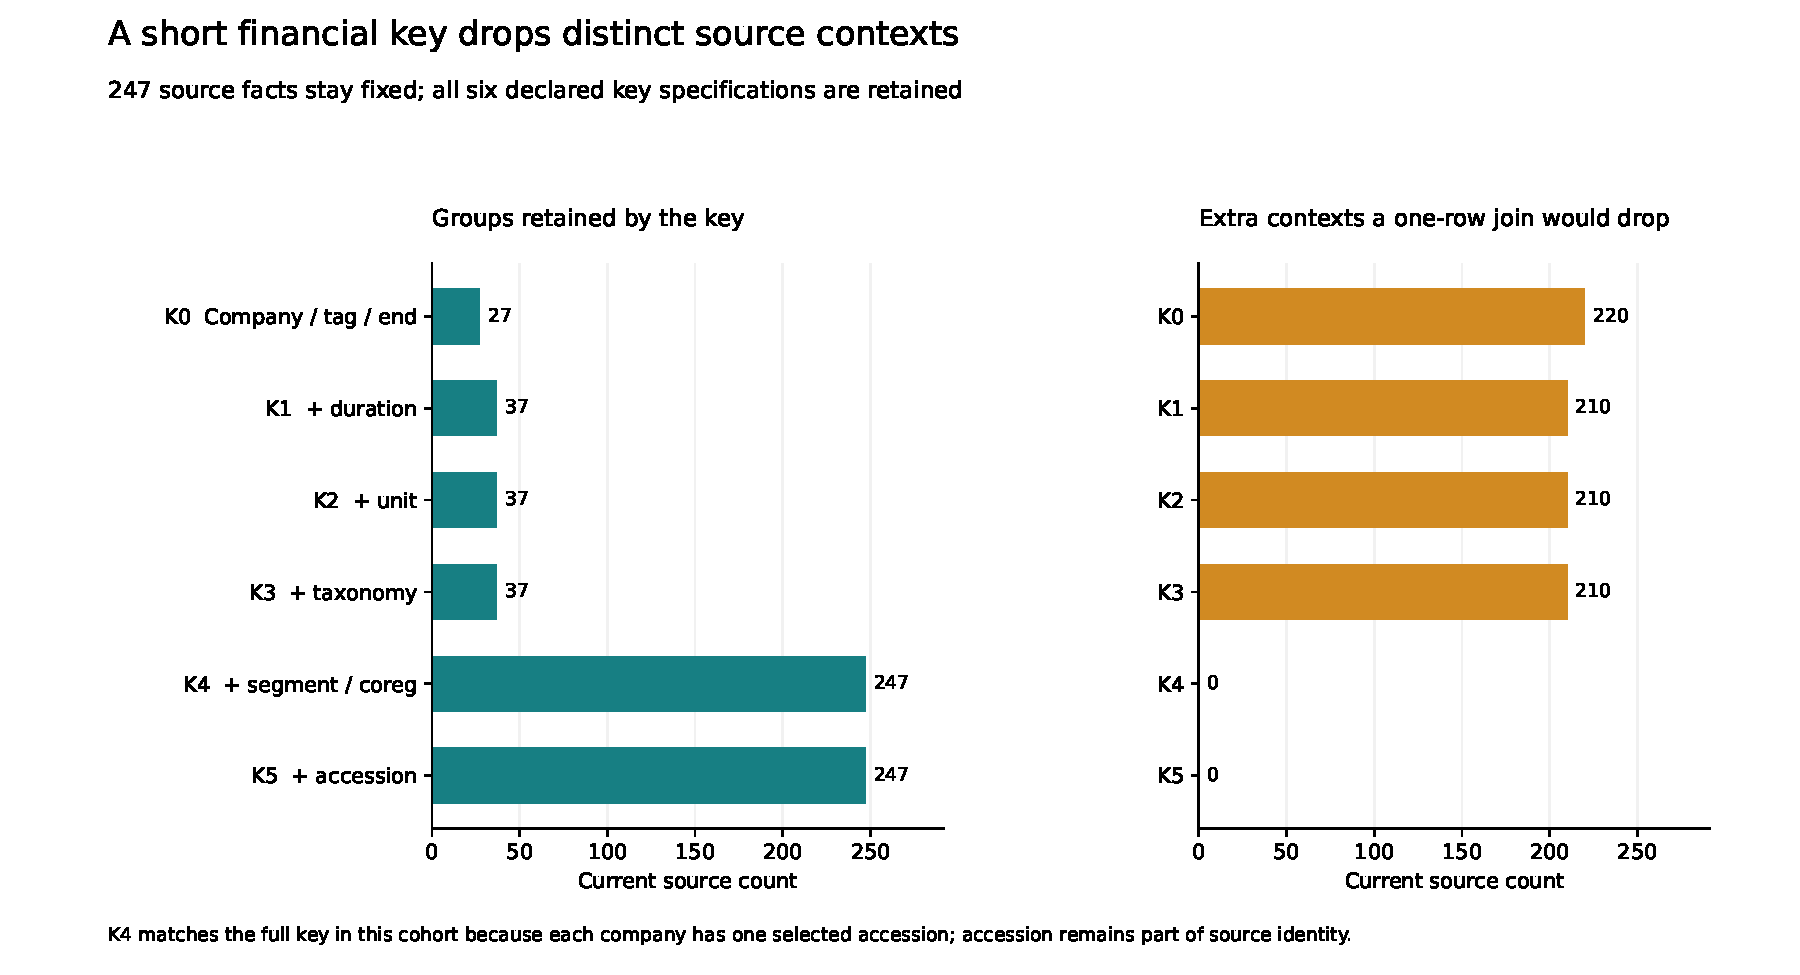
\includegraphics[width=9.4in,height=6.25in,keepaspectratio]{images/key_retention.pdf}\end{center}
\end{landscape}
\begin{landscape}
{\large\bfseries All omitted-context accounts\par}
\begin{center}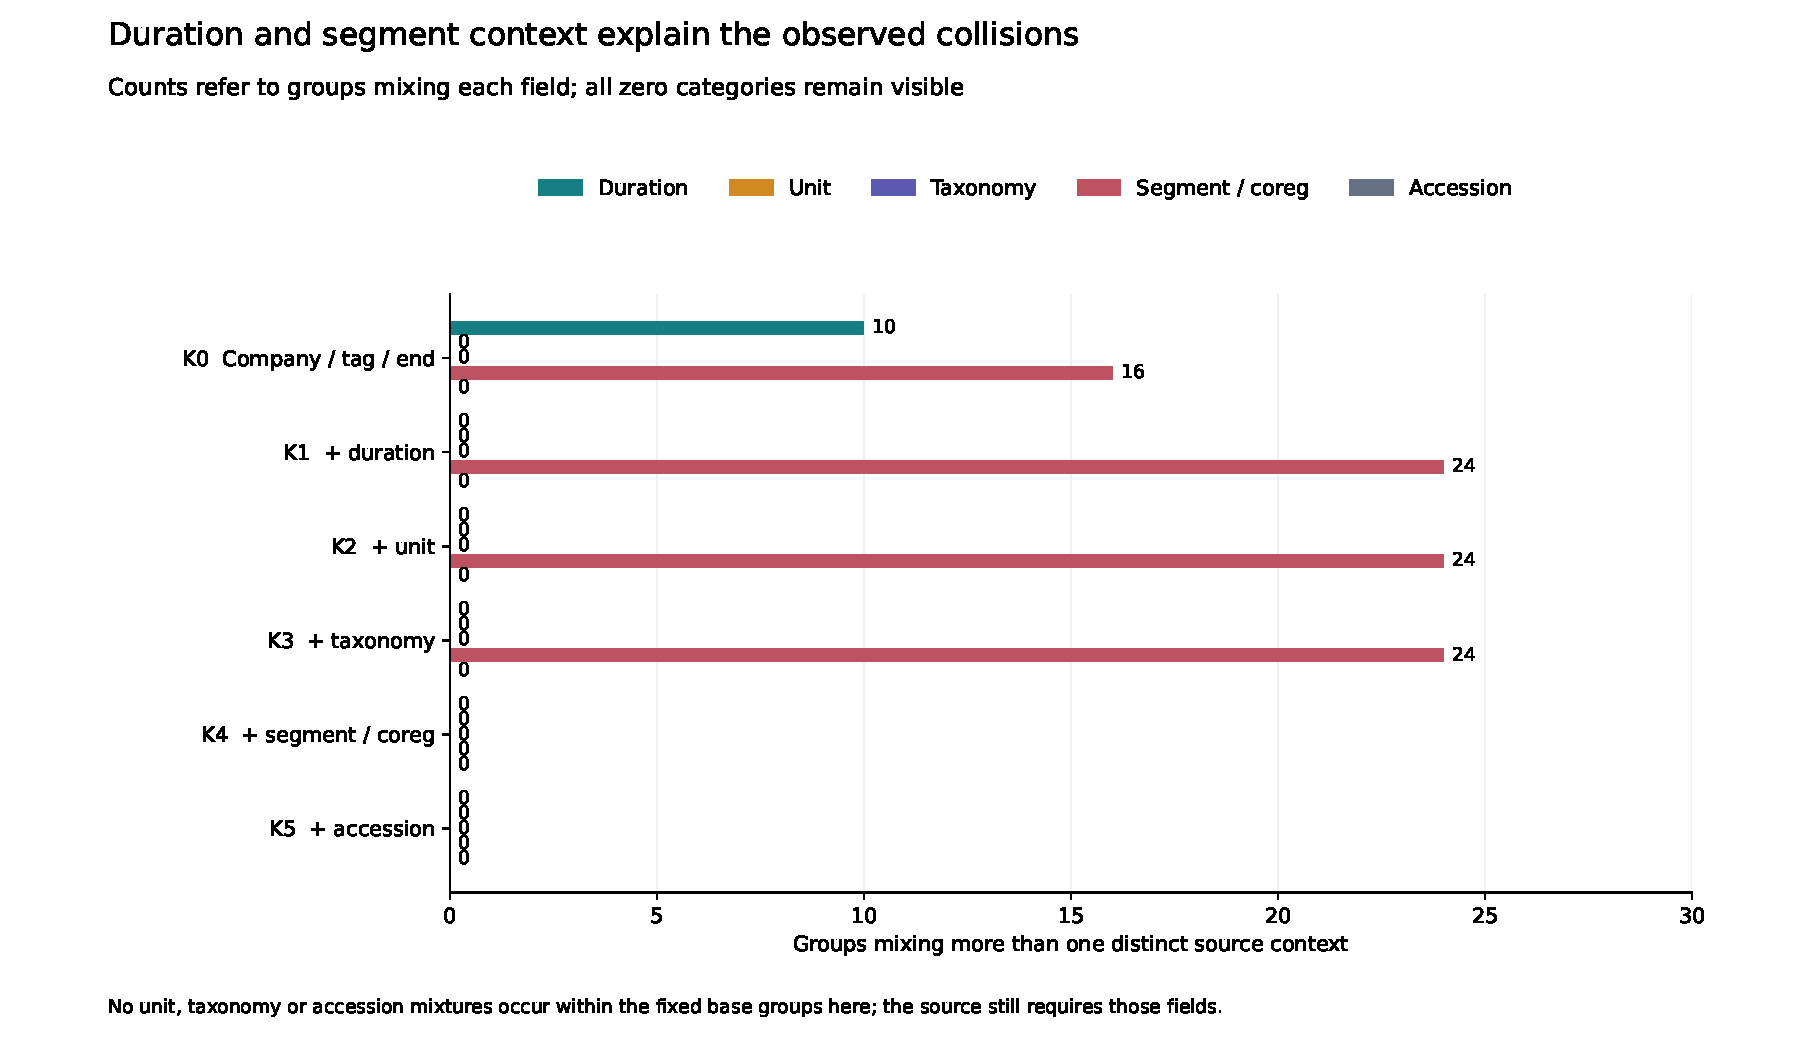
\includegraphics[width=9.4in,height=6.25in,keepaspectratio]{images/context_collisions.pdf}\end{center}
\end{landscape}
\begin{landscape}
{\large\bfseries Numeric disagreement and interpretation\par}
\begin{center}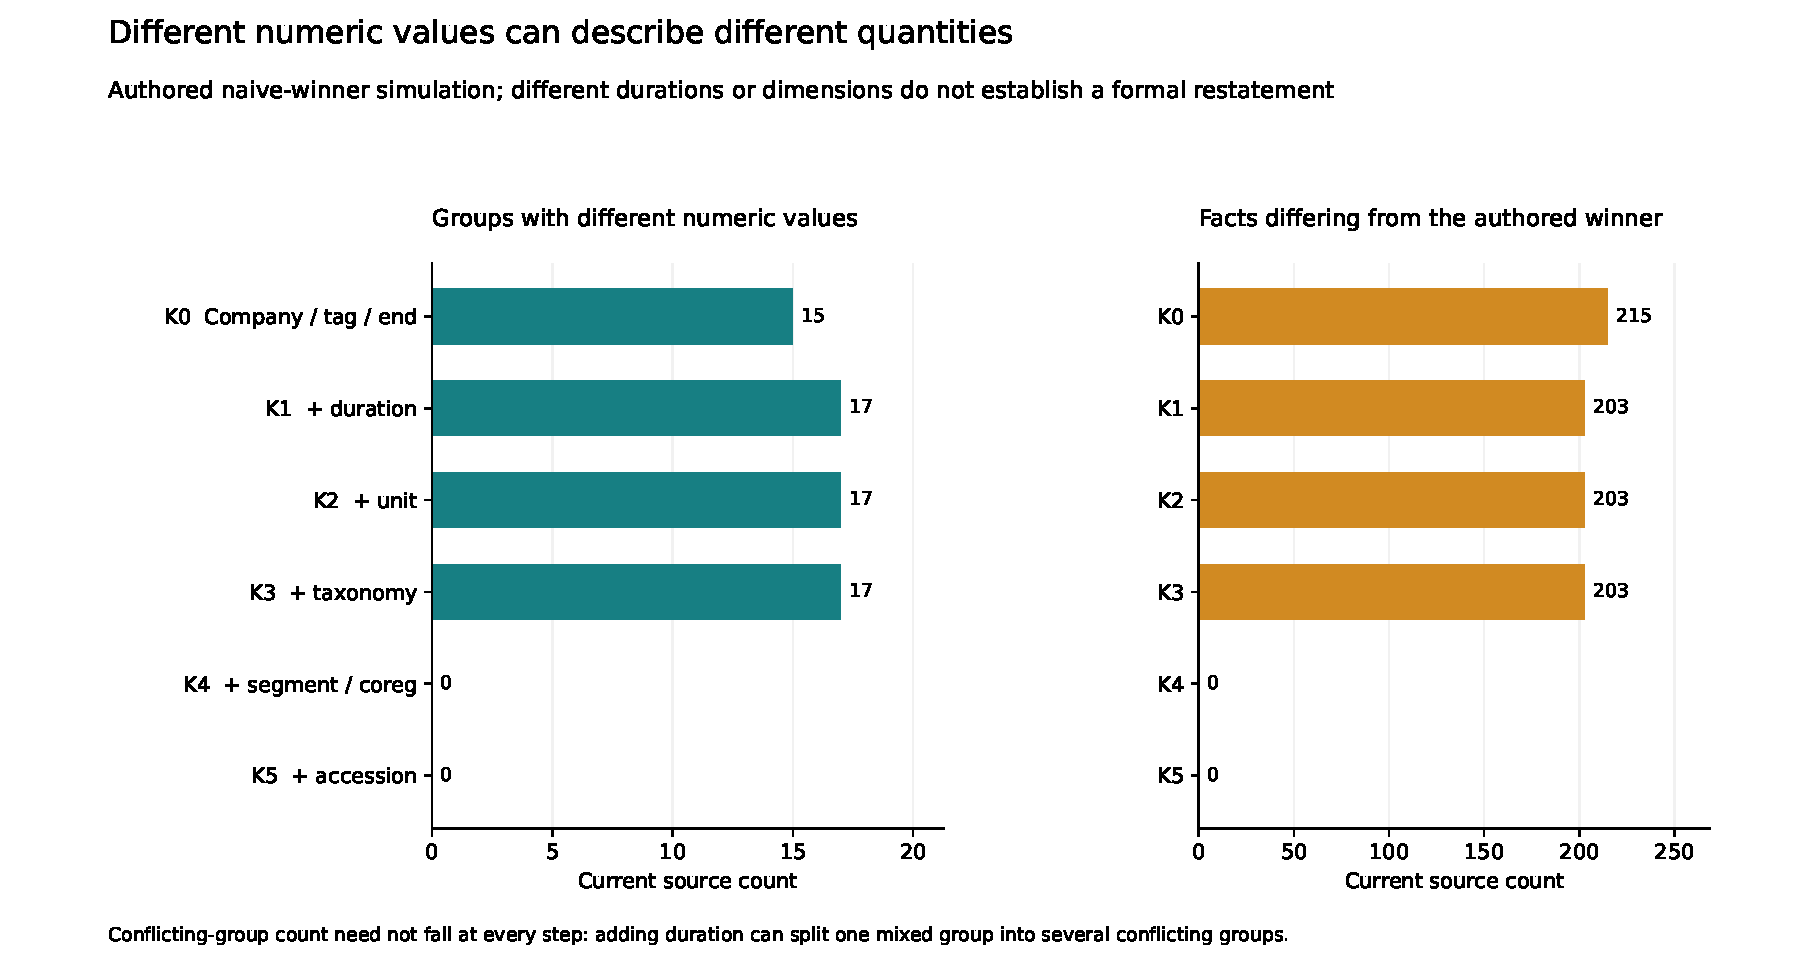
\includegraphics[width=9.4in,height=6.25in,keepaspectratio]{images/numeric_disagreement.pdf}\end{center}
\end{landscape}
\end{document}
